%
% File naaclhlt2009.tex
%
% Contact: nasmith@cs.cmu.edu

\documentclass[english,11pt]{article}
\usepackage{naaclhlt2009}
\usepackage{times}
\usepackage{latexsym}
\usepackage{amsthm} 
\usepackage{amsmath}
\usepackage{amssymb}
\usepackage[authoryear]{natbib}
\usepackage{multirow}
\usepackage{subfig}

\setlength\titlebox{6.5cm}    % Expanding the titlebox

\theoremstyle{plain}
\theoremstyle{plain} 
\newtheorem{thm}{Theorem}
  \theoremstyle{plain}
  \newtheorem{algorithm}[thm]{Algorithm}

\usepackage{babel}

% just a working title
\title{Optimal IBM Model 4 Decoding Revisited}

% \author{Joakim Nivre \\
%   School of Mathematics and Systems Engineering \\
%   V\"{a}xj\"{o} University \\
%   SE-35195, V\"{a}xj\"{o}, Sweden \\
%   {\tt nivre@msi.vxu.se} \And
%   Noah A. Smith \\
%   Language Technologies Institute \\
%   Carnegie Mellon University \\
%   Pittsburgh, PA 15213, USA\\
%   {\tt nasmith@cs.cmu.edu}}

\date{}

\begin{document}
\maketitle
\begin{abstract}
  This document contains the instructions for preparing a camera-ready
  manuscript for the proceedings of NAACL HLT 2009. The document itself conforms
  to its own specifications, and is therefore an example of what
  your manuscript should look like.  Authors are asked to conform to
  all the directions reported in this document.
\end{abstract}

\section{Introduction}
\label{sec:introduction}

Semantic Role Labelling~\citep[SRL, ][]{marquez08srl} is generally understood as 
the task of identifying and classifying the semantic arguments and modifiers of 
the predicates mentioned in a sentence. For example, in the case of the 
following sentence:\footnote{``Haag plays Elianti'' is a segment of a sentence in 
training corpus.}
\begin{quote}
\begin{center}
    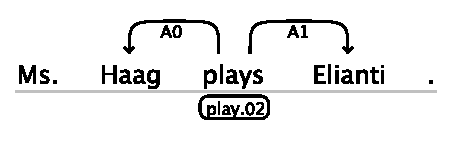
\includegraphics[scale=.63]{haag-example}
\end{center}
\end{quote}
we are to find out that for the predicate token {}``plays'' with sense ``play a 
role'' (play.02) the phrase headed by the token {}``Haag'' is referring to the 
player (A0) of the play event, and the phrase headed by the token {}``Elianti''  
is referring to the role (A1) being played. SRL is considered as a key task for 
applications that are required to answer questions such as {}``Who'', {}``What'', {}``Where'', etc.  

In this paper we introduce a Markov Logic~\citep[ML,][]{richardson06mln} approach to multi-lingual
SRL. We present a brief introduction to ML in 
section \ref{sec:markovlogic}.  At the core of ML are Markov Logic Networks~(MLN): sets of weighted First Order 
Logic (FOL) formulae. One attractive feature of the ML 
framework is that we can divide FOL formulae into subsets that serve as re-usable ``modules''. 
With this in mind we define MLN modules which capture the different stages of 
the task: argument identification, argument classification, and sense 
disambiguation. We also define modules for some of the language specific aspects of 
the task. We present all our ML modules in section 
\ref{sec:model}. These modules are the building blocks that we use to create 
MLNs for specific languages. We present our experiments and results for each of 
the languages of the task in section \ref{sec:results}.
% In section \ref{sec:analysis} we present some error analysis.



% we could wrap a supersection around the following 3 sections, but that 
% takes extra space. 

\section{IBM Model 4} 
\label{sec:ibm-model-4}
In this paper we focus on the translation model defined by IBM Model
4~\citep{model4}.  Translation using IBM Model 4 is performed by
treating the translation process a noisy-channel model where the
probability of the English sentence given a French sentence is,
$P(\mathbf{e}|\mathbf{f}) = P(\mathbf{f}|\mathbf{e}) \cdot
P(\mathbf{e})$, where $P(\mathbf{e}$) is a language model of English.
IBM Model 4 defines $P(\mathbf{f}|\mathbf{e})$ and models the
translation process as a generative process of how a sequence of
target words (in our case French or German) is generated from a
sequence of source words (English).

The generative story is as follows.  Imagine we have an English
sentence, $\mathbf{e} = e_1, \dots,e_l$ and along with a NULL word
($e_o$) and French sentence, $\mathbf{f} = f_1, \dots, f_m$.  First a
fertility is drawn for each English word (including the NULL symbol).
Then, for each $e_i$ we then independently draws a number of French
words equal to $e_i$'s fertility.  Finally we process the English
source tokens in sequence to determine the positions of their
generated French target words.  We refer the reader to~\cite{model4}
for full details.



%%% Local Variables: 
%%% mode: latex
%%% TeX-master: "ilp-mt"
%%% End: 
 
 
\section{Integer Linear Programming Formulation}
\label{sec:ilp}

\global\long\def\source{\mathbf{e}}
\global\long\def\target{\mathbf{f}}
\global\long\def\align{\mathbf{a}}
\global\long\def\start{\text{START}}
\global\long\def\stop{\text{END}}
\global\long\def\null{\text{NULL}}
\global\long\def\sourceset{S}


Given a trained IBM model 4, and a French sentence $\target$ we need
to find the English sentence $\source$ and alignment $\align$ with
maximal $p\left(\align,\source|f\right)\backsimeq p\left(\source\right)\cdot p\left(\align,\target|\source\right)$.
\citet{germann01fast} presented an Integer Linear Programming~(ILP) formulation of this problem. In this section we will give a very high-level description of this ILP formulation.%
\footnote{Note that our formulation differs slightly because we use a first order modelling
language that imposed certain restrictions on the type of constraints
allowed.%
} For brevity we refer the reader to the original work for details of the ILP formulation. 

In their ILP formulation an English translation is represented as a path through a set of English candidate tokens. A set of binary variables denote whether or not certain token pairs are directly connected through this path. Among constraints which guarantee that each French word has exactly one English word that generates it, the program also contains an exponential number of constraints that forbid each possible cycle the variables can represent. It is this set of constraints that renders decoding with ILP difficult. 

 





\section{Cutting Plane Algorithm}
\label{sec:cutting-plane}
\global\long\def\y{\mathbf{y}}


The ILP program above has an exponential number of (cycle)
constraints. Hence, simply passing the ILP to an off-the-shelf ILP
solver is not practical for all but the smallest sentences. For this
reason \citet{GermannFast04} only consider sentences of up to eight
tokens. However, recent work~\citep{riedel06incremental} has shown
that even exponentially large decoding problems may be solved
efficiently using ILP solvers if a Cutting-Plane
Algorithm~\citep{dantzig54solution} is used.%
\footnote{It is worth mentioning that Cutting Plane Algorithms have
  been successfully applied for solving very large instances of the
  Travelling Salesman Problem, a problem essentially equivalent to the
  decoding in IBM Model 4.}

% In the following we will present a Cutting Plane algorithm for IBM
% Model 4:
% \begin{enumerate}
% \item Construct ILP $I$ without cycle constraints

% \begin{enumerate}
% \item \textbf{do}

% \begin{enumerate}
% \item solve $I$ and assign to solution $\y$
% \item find cyclic paths in solution $\y$
% \item add corresponding cycle constraints to $I$
% \end{enumerate}
% \textbf{until} no more cyclic paths can be found

% \item \textbf{return} $\y$
% \end{enumerate}
% \end{enumerate}
A Cutting-Plane Algorithm starts with a subset of the complete set of
constraints. In our case this subset contains all but the
(exponentially many) cycle constraints. The corresponding ILP is
solved by a standard ILP solver, and the solution is inspected for
cycles. If it contains no cycles, we have found the true optimum: the
solution with highest score that does not violate any constraints. If
the solution does contain cycles, the corresponding constraints are
added to the ILP which is in turn solved again. This process is
continued until no more cycles can be found.

% It is difficult to make claims about a guaranteed worst-case runtime
% (or number of iterations) of this algorithm. However, if the linear
% scoring function (in other words, the translation model and language
% model parameters) already provides a preference for cycle-free solutions,
% we can expect this algorithm to be efficient. For example, if we assume
% that the translation/distortion model has a very strong preference
% for monotonic solutions then clearly the highest scoring solution
% is likely to be cycle-free.




%%% Local Variables: 
%%% mode: latex
%%% TeX-master: "ilp-mt"
%%% End: 


\section{Evaluation}
\label{sec:evaluation}

Table \ref{tbl:results} shows the results of our systems for the CoNLL 2008 development set and the WSJ and brown test sets. The scores are calculated using the semantic evaluation metric of the CoNLL-08 shared task \citep{surdeanu08conll}. This metric measures the precision, recall and $F_1$ score of the recovered semantic dependencies. A semantic dependency is created for each predicate and its arguments, the label of such dependency is the role of the argument. Additionally, there is a semantic dependency for each predicate and a $ROOT$ argument which has the sense of the predicate as label.
%This metric not only measures the $F_1$ score in terms of the semantic arguments, but also includes the accuracy of the predicted predicate senses.  


%%Need more detailed explanation 
%The table also includes results from two existing approaches. The first one, Vicrey, was the winning system in the CoNLL 2008 shared task open track (here MALT parse trees were given). The second one, Johansson, won the closed track of the same competition (here parse trees had to be predicted, too). The results for their systems were taken from the overview paper~(cite) and only show the $F_1$ scores for the verbal/PropBank predicates.\footnote{Extracted from Table 16 of the mentioned paper.}

To put these results into context, let us compare them to those of the participants of the CoNLL 2008 shared task (see the last three rows of table \ref{tbl:results}).\footnote{Results of other systems were extracted from Table 16 of the shared task overview paper \citep{surdeanu08conll}.} Our best model, Bottom-up, would reach the highest $F_1$ WSJ score, and second highest Brown score, for the open track. Here the best-performing participant was \citet{vickrey08applying}. 

Table \ref{tbl:results} also shows the results of the best~\citep{johansson08dependency} and fourth best system~\citep{zhao08parsing} of the closed track. We note that we do significantly worse than \citet{johansson08dependency}, and roughly equivalent to \citet{zhao08parsing}; this places us on the fourth rank of 19 participants. However, note that all three systems above us, as well as  \citet{zhao08parsing}, use parsers with at least about 90\% (unlabelled) accuracy on the WSJ test set (Johansson's parser has about 92\% unlabelled accuracy).\footnote{Since our parses use a different label set we could not compare labelled accuracy.} By contrast, with about 87\% unlabelled accuracy our parses are significantly worse.   

Finally, akin to \citet{riedel08collective} we observe that the bottom-up joint model performs better than the full joint model. % Hence we will focus on this model in the remainder of this paper.

%It would reach the 4th highest score (for both WSJ and Brown) for the closed track, only beaten by systems that use 
%use highly optimized (ensemble-based, 2nd order, etc.) dependency parsers as input. In the closed track the highest score was obtain by \citet{johansson08dependency} system. Note that this comparison is based only on the results for verbal predicates.


\begin{table}[ht]
    \centering
    \begin{tabular}{|p{3.0cm}|c|c|c|}\hline
        System                    & Devel      & WSJ       & Brown \\\hline 
        Full                      & $76.93$  & $79.09$ & $67.64$ \\
        % 112508_235756
        Bottom-up                 & $77.96$  & $80.16$ & $68.02$ \\
        % 112708_202510
        Bottom-up (-arg)          & $77.57$  & $79.37$ & $66.70$ \\
        % 112908_202731
        Pipeline                  & $75.69$  & $78.19$ & $64.66$ \\
        % 112508_223504
        \hline
        Vickrey                   &   N/A    & $79.75$ & $69.57$ \\
        Johansson                 &   N/A    & $86.37$ & $71.87$ \\
        Zhao                      &   N/A    & $79.40$ & $66.38$ \\
        \hline
    \end{tabular}
    \caption{Semantic $F_1$ scores for our systems and three CoNLL 2008 shared 
    task participants. Bottom-up model is statistically significant better than 
    the rest (i.e., $\rho \le 0.05$.)} %IV-
    %Systems that do not explicitely model the $isArgument$ decisions are marked with (-arg).}
    \label{tbl:results}
\end{table}

% number of assigments:
% full          18621
% bottom-upi    17611
% bottom-up (-arg) 17545
% pipeline 18342

% WSJ
% Siginificanse score for bottom-up model
% bottom-up vs full = n+ 468, n- 276, p <= 2.53e-12
% bottom-up vs bottom-up (-arg) = n+ 255, n- 447, p <= 5.68e-13
% bottom-up vs pipeline = n+ 500, n- 600, p <= 0.00284
% full vs pipeline = n+ 621, n- 339, p <= 1.22e-19
% botto-up (isarg) vs pipeline = n+ 640, n- 548, p <= 0.00829

% Brown

%% Unlabelled dependency accuracy for WSJ
% We (Charniak): 86.77%
% Johansson: 92.45
% che: 90.03
% ciaramita: 90.20
% zhao: 89.86 


\subsection{Joint Model vs. Pipeline}
Table \ref{tbl:results} suggests that by including sense disambiguation into the joint model (as is the case for all systems but the pipeline) significant improvements can be gained. Where do these improvements come from? We tried to answer this question by taking a closer look at how accurately the pipeline predicts the $isPredicate$, $isArgument$, $hasRole$, $role$ and $sense$ relations, and how this compares to the result of the joint full model.

Table \ref{tbl:predicates} shows that the joint model mainly does better when it comes to predicting the right predicate senses. This is particularly true for the case of the Brown corpus---here we gain about 10\% points. These results suggest that a more joint approach may be particularly useful in order to increase the robustness of an SRL system in out-of-domain scenarios \footnote{All scores in the full model when compared with the pipeline model are statistically significant with exception of the $isPredicate$ predicate for the WSJ test set.}.

% The role labelling in figure \ref{fig:jointSense} illustrates how the joint model overcomes a limitation of the pipeline approach. Here the argument identification and classification stage of the pipeline has wrongly picked `You'' the A0 role and ``lawyer'' the A2 role of the predicate ``realize''. Because the role A2 (``created from'') only appears in the  02 (``create'') sense of ``realize'', the sense disambiguation stage wrongly selects the 02 instead of the corrent 01 (``come to know'') sense. In contrast, the joint full model knows that by simply dropping ``You'' as argument all together and changing the A2 to an A0 label, the sense 01 becomes a very suitable and consistent choice (even though the role labelling itself might be slightly less likely).

\begin{table}[ht]

    \centering
    \begin{tabular}{|c|c|c|c|c|}\hline
      & \multicolumn{2}{c|}{WSJ} & \multicolumn{2}{c|}{Brown}\\
                                  & Pipe.  &  Fu.   & Pipe.  &  Fu. \\\hline 
        \emph{isPredicate}        & $96.6$ & $96.5$ & $92.2$ & $92.5$\\
        \emph{isArgument}         & $90.3$ & $90.6$ & $85.9$ & $86.9$ \\
        \emph{hasRole}            & $88.0$ & $87.9$ & $83.6$ & $83.8$ \\
        \emph{role}               & $75.4$ & $75.5$ & $64.2$ & $64.6$ \\
        \emph{sense}              & $85.5$ & $88.5$ & $67.3$ & $77.1$ \\\hline
    \end{tabular}
    \caption{$F_1$ scores for M predicates; Pipe. refers to the Pipeline system, Fu. to the full system.}
    \label{tbl:predicates}
\end{table}

% WSJ
%isPredicate, n+ 49, n- 53, p <= 0.766
 %POS: 49
 %NEG: 53
%isArgument, ??? 
 %POS: 10870
 %NEG: 4
%frameLabel, n+ 253 , n- 111, p <= 1.48e-13
 %POS: 253
 %NEG: 111
%hasLabel, n+ 143, n- 346, p <= 6.66e-20
 %POS: 346
 %NEG: 143
%role, n+ 400, n- 226, p <= 4.73e-12
 %POS: 400
 %NEG: 226

%using conll08 files:
%isArgument, n+ 255, n- 114, p <= 3.17e-13
% POS: 255
% NEG: 114

% Brown
%isPredicate, n+ 35, n- 17, p <= 0.0175
 %POS: 35
 %NEG: 17
%isArgument, ??
 %POS: 1285
 %NEG: 1
%frameLabel, n+ 67, n- 16, p <= 1.39e-08
 %POS: 67
 %NEG: 16,
%hasLabel, n+ 65, n- 25, p <= 2.97e-05
 %POS: 65
 %NEG: 25
%role, n+ 59, n- 26, p <= 0.000447
 %POS: 59
 %NEG: 26

%Using conll08 files
%isArgument, n+ 60, n- 21, p <= 1.69e-05
% POS: 60
% NEG: 21



% \begin{figure}
% \begin{center}
%     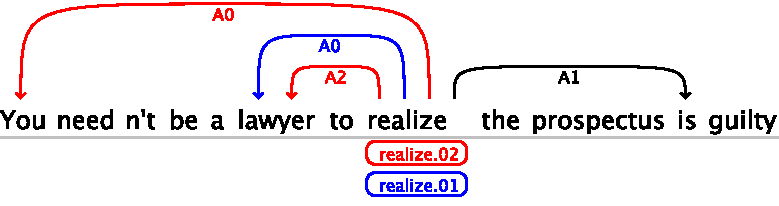
\includegraphics[scale=.58]{joint-sense-example}
% \end{center}
% \caption{Fragment of sentence in the development set that the pipeline model gets wrong: it picks the wrong sense (``02'') for ``realize'' and falsely assigns ``You'' the A0 role and ``lawyer'' the A2 role.}
% \label{fig:jointSense}
% \end{figure}


% I don't quite understand why we did isArg vs no isArg :-S. Maybe, too late to
% bring the issue. I just put two columns, if I put dev and brown, they get too
% big.
% SR: Huh? Without isArg we wouldn't need to jointly predict args for ALL predicates of one sentence. So this is to justify the joint model, and the fact that we explicitely model isArgument (different from all other SRL models I know). 

\subsection{Modelling if a Token is an Argument}
In table \ref{tbl:results} we also observe that improvements can be made if we explicitly model the decision whether a token is a semantic argument of some predicate or not. As we mentioned in section \ref{sec:model}, this aspect of our model requires us to jointly perform inference for all predicates of a sentence, and hence our results justify the per-sentence SRL approach proposed in this paper.

In order to analyse where these improvements come from, we again list our results on a per-SRL-predicate basis. Table \ref{tbl:isArg} shows that by including the $isArgument$ predicate and the corresponding formulae we gain around 0.6\% and 1.0\% points across the board for WSJ and Brown, respectively. As shown in table \ref{tbl:results}, these improvements result in about 1.0\% improvements for both WSJ and Brown in terms of the CoNLL 2008 metric. Hence, an explicit model of the ``is an argument'' decision helps the SRL at all levels \footnote{All scores in the bottom-up when compared with the version without the $isArgument$ predicate are statistically significant with exception of the $sense/2$ predicate for the Brown test set.}.

How the $isArgument$ helps to improve the overall role labelling score can be illustrated with the example in figure \ref{fig:isArg}. Here the model without a hidden $isArgument$ predicate fails to attach the preposition ``on'' to the predicate ``start.01'' (here 01 refers to the sense of the predicate). Apparently the model has not enough confidence to assign the preposition to either ``start.01'' or ``get.03'', so it just drops the argument altogether. However, because the $isArgument$ model knows that most prepositions have to be modifying some predicate, pressure is created that forces a decision between the two predicates. And because for the role model ``start.01'' looks like a better fit than ``get.03'', the correct attachment is found.

%%example
\begin{figure}
\begin{center}
    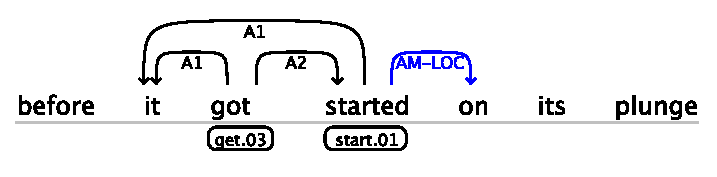
\includegraphics[scale=.62]{is-arg-example}
\end{center}
\caption{Segment of the CoNLL 2008 development set for which the bottom-up model w/o $isArgument$ predicate fails to attach the preposition ``on'' as an ``AM-LOC'' for ``started''. The joint bottom-up model attaches the preposition correctly.}
\label{fig:isArg}
\end{figure}


\begin{table}[ht]

    \centering
    \begin{tabular}{|c|c|c|c|c|}\hline
      & \multicolumn{2}{c|}{WSJ} & \multicolumn{2}{c|}{Brown}\\
                                  & w/o     & w/     & w/o    & w/  \\\hline 
        \emph{isPredicate}        & $96.3$  & $96.5$ & $91.4$ & $92.5$\\
%%        \emph{isArgument}         &         & $86.6$ &        & $86.6$ \\
        \emph{hasRole}            & $87.1$  & $87.7$ & $82.5$ & $83.6$ \\
        \emph{role}               & $76.9$  & $77.5$ & $65.2$ & $66.2$ \\
        \emph{sense}              & $88.3$  & $89.0$ & $76.1$ & $77.5$ \\\hline
    \end{tabular}
    \caption{$F_1$ scores for ML predicates; w/o refers to a Bottom-up system without isArgument predicate, w/ refers to a Bottom-up system with isArgument predicate.}
    \label{tbl:isArg}
\end{table}

% WSJ
%isPredicate, n+ 56, n- 17, p <= 5.27e-06
 %POS: 56
 %NEG: 17
%isArgument
 %POS: 10800
 %NEG: 0
%frameLabel,n+ 100, n- 50, p <= 6.31e-05
 %POS: 100
 %NEG: 50
%hasLabel, n+ 286, n- 174, p <= 2.28e-07
 %POS: 286
 %NEG: 174
%role, n+ 293, n- 196, p <= 1.42e-05
 %POS: 293
 %NEG: 196

%Brown
% isPredicate, n+ 47, n- 7, p <= 2.29e-08
% POS: 47
% NEG: 7
%isArgument
% POS: 1280
% NEG: 0
%frameLabel,n+ 21, n- 12, p <= 0.163
% POS: 21
% NEG: 12
%hasLabel, n+ 55, n- 33, p <= 0.0246
% POS: 55
% NEG: 33
%role, n+ 58, n- 32, p <= 0.00805
% POS: 58
% NEG: 32


\subsection{Efficiency}
In the previous sections we have shown that our joint model indeed does better than an equivalent pipeline system. However, usually most joint approaches come at a price: efficiency. Interestingly, in our case we observe the opposite: our joint model is actually faster than the pipeline. This can be seen in table \ref{tbl:nocpi}, where we list the time it took for several different system to process the WSJ and Brown test corpus, respectively. When we compare the times for the bottom-up model to those of the pipeline, we note that the joint model is twice as fast. While the individual stages within the pipeline may be faster than the joint system (even when we sum up inference times), extracting results from one system and feeding them into another creates overhead which offsets this potential reduction.  

Table \ref{tbl:nocpi} also lists the run-time of a bottom-up system that solves the inference problem by fully grounding the Markov Network that the Markov Logic (ML) model describes, mapping this network to an Integer Linear Program, and finding the most likely assignment using an ILP solver. This system (Bottom-up (-CPI)) is four times slower than the equivalent system that uses Cutting Plane Inference  (Bottom-up). This suggests that if we were to implement the same joint model using ILP instead of ML, our system would either be significantly slower, or we would need to implement a Cutting Plane algorithm for the corresponding ILP formulation---when we use ML this algorithm comes ``for free''. 
% \begin{table}[ht]

%     \centering
%     \begin{tabular}{|p{2.5cm}|c|c|c|}\hline
%         System                           & Training & Testing   & Testing \\
%                                          &          & WSJ       & Brown   \\\hline 
%         Full model                       & $5.1$h   & $9.2$m    & $1.5$m  \\
%         Bottom-up                        & $4.3$ih  & $9.5$m    & $1.6$m  \\
%         Full model w/o \emph{isArgument} &          &           &         \\
%         Bottom-up  w/o \emph{isArgument} & $3.9$h   & $12.5$m   & $1.5$m \\
%         Pipeline                         & $5.0$h   & $18.9$m   & $2.9$m \\\hline
%     \end{tabular}
%     \caption{Testing and training times for the systems.}
%     \label{tbl:times}
% \end{table}

\begin{table}[ht]

    \centering
    \begin{tabular}{|p{3.0cm}|c|c|}\hline
        System                           & WSJ       & Brown   \\\hline 
        Full                             & $9.2$m    & $1.5$m  \\
        Full (-CPI)                      & $38.4$m   & $7.47$m  \\
        Bottom-up                        & $9.5$m    & $1.6$m  \\
        Bottom-up (-CPI)                 & $38.8$m   & $6.9$m  \\
        Pipeline                         & $18.9$m   & $2.9$m  \\\hline
    \end{tabular}
    \caption{Testing times for full model and bottom-up when CPI algorithm is
    not used. The WSJ test set contains 2414 sentences, the Brown test set 426. Our best systems thus takes on average 230ms per WSJ sentence (on a 2.4Ghz system). }
    \label{tbl:nocpi}
\end{table}


%7. Results
%7.1 Joint/Bottom-up vs pipeline
%- Illustrate that we get dramatic improvements in sense
%disambiguation, but not in other parts. Stress effect on Brown
%- Show table that compares isPredicate & role & frameLabel results for
%pipeline vs joint models (this would show that no gain in isPredicate
%and role, but in frameLabel)
%- Give example from dev-set
%7.2 With isArg vs without isArg
%- illustrate that we get improvements in all sections
%- show table that compares individual predicate scores (dev, wsj,
%brown) for isArg vs w/o isArg
%- maybe find example?
%7.3 (Maybe) Full vs Bottom-up again (maybe not because in other paper)
%7.4 Efficiency
%- Illustrate that training the model jointly comes at no extra cost
%(we can train as fast/faster with the joint bottom up model than with
%a pipeline)
%- Illustrate that inference is much more efficient when compared to an
%equivalent ILP-only system (which is basically the w/o CPI system)
%- Can we also have a sentence/second column for testing?
%
%
%Pipeline
%**************
%         isPredicate    : 0.958,0.959,0.958,0.959,0.959
%          isArgument    : 0.890,0.892,0.891,0.891,0.891
%            hasLabel    : 0.870,0.873,0.872,0.872,0.872
%                role    : 0.706,0.718,0.720,0.722,0.723
%          frameLabel    : 0.834,0.842,0.841,0.841,0.841
%
%         isPredicate    : 0.966,0.922
%          isArgument    : 0.903,0.859
%            hasLabel    : 0.880,0.836
%                role    : 0.754,0.642
%          frameLabel    : 0.855,0.673
%
%Times :
%trainning (hrs):
%stage1= 0.76
%stage2= 3.42
%stage3= 0.84
%total = 5.02
%testing:
%stage1: 5.44m, 42.68s
%stage2: 7.56m, 1.27m 
%stage3: 5.96m, 54.03s
%total: 18.96,  2.90m
%
%
%WSJ
%  Labeled precision:          (10284 + 4521) / (13021 + 5321) * 100 = 80.72 %
%  Labeled recall:             (10284 + 4521) / (14269 + 5260) * 100 = 75.81 %
%  Labeled F1:                 78.19
%
%Brown
%  Labeled precision:          (1335 + 555) / (1986 + 846) * 100 = 66.74 %
%  Labeled recall:             (1335 + 555) / (2210 + 804) * 100 = 62.71 %
%  Labeled F1:                 64.66
%
%
%
%Full model
%**************
%         isPredicate    : 0.958,0.959,0.958,0.958,0.958
%          isArgument    : 0.894,0.895,0.895,0.895,0.895
%            hasLabel    : 0.865,0.868,0.869,0.869,0.869
%                role    : 0.703,0.713,0.720,0.724,0.727
%          frameLabel    : 0.870,0.874,0.878,0.877,0.878
%
%         isPredicate    : 0.965,0.923
%          isArgument    : 0.906,0.869
%            hasLabel    : 0.879,0.838
%                role    : 0.755,0.646
%          frameLabel    : 0.885,0.771
%
%Times:
%Training :5.09 hrs
%Testing:
%WSJ          9.15m 
%Brown        1.58m 
%
%
%WSJ
%  Labeled precision:          (10423 + 4664) / (13348 + 5273) * 100 = 81.02 %
%  Labeled recall:             (10423 + 4664) / (14269 + 5260) * 100 = 77.25 %
%  Labeled F1:                 79.09
%
%Brown
%  Labeled precision:          (1369 + 621) / (2063 + 807) * 100 = 69.34 %
%  Labeled recall:             (1369 + 621) / (2210 + 804) * 100 = 66.03 %
%  Labeled F1:                 67.64
%
%
%Full model w/o isArg (NOTE: not with new formula2/ we need it with bottom-up model as well)
%**************
%
%       isPredicate      : 0.955,0.955,0.954,0.955,0.955
%            hasLabel    : 0.860,0.863,0.866,0.865,0.865
%                role    : 0.710,0.722,0.727,0.730,0.730
%          frameLabel    : 0.869,0.874,0.875,0.876,0.875
%
%         isPredicate    : 0.963,0.910
%            hasLabel    : 0.872,0.818
%                role    : 0.752,0.638
%          frameLabel    : 0.878,0.761
%
%Times (hrs)
%Training: 4.58
%Testing:
%WSJ       9.53m 
%Brown     1.43m 
%
%
%
%WSJ
%  Labeled precision:          (10308 + 4615) / (13132 + 5257) * 100 = 81.15 %
%  Labeled recall:             (10308 + 4615) / (14269 + 5260) * 100 = 76.41 %
%  Labeled F1:                 78.71
%
%Brown
%  Labeled precision:          (1324 + 609) / (1973 + 797) * 100 = 69.78 %
%  Labeled recall:             (1324 + 609) / (2210 + 804) * 100 = 64.13 %
%  Labeled F1:                 66.84
%
%
%
%Bottom up
%**************
%         isPredicate    : 0.958,0.960,0.960,0.960,0.959
%          isArgument    : 0.893,0.895,0.895,0.894,0.894
%            hasLabel    : 0.867,0.870,0.869,0.870,0.869
%                role    : 0.728,0.738,0.743,0.746,0.747
%          frameLabel    : 0.872,0.878,0.885,0.887,0.883
%
%         isPredicate    : 0.965,0.925
%          isArgument    : 0.904,0.866
%            hasLabel    : 0.877,0.836
%                role    : 0.775,0.662
%          frameLabel    : 0.890,0.775
%
%Times:
%Training 4.26 hrs
%Testing:
%WSJ          9.53m 
%Brown        1.55m 
%
%WSJ
%  Labeled precision:          (10315 + 4590) / (12349 + 5262) * 100 = 84.63 %
%  Labeled recall:             (10315 + 4590) / (14269 + 5260) * 100 = 76.32 %
%  Labeled F1:                 80.26
%
%Brown
%  Labeled precision:          (1327 + 591) / (1836 + 812) * 100 = 72.43 %
%  Labeled recall:             (1327 + 591) / (2210 + 804) * 100 = 63.64 %
%  Labeled F1:                 67.75
%
%
%NO CPI 
%**************
%         isPredicate    : 0.959,0.958,0.958,0.957,0.957
%          isArgument    : 0.894,0.896,0.895,0.895,0.893
%            hasLabel    : 0.867,0.869,0.870,0.868,0.867
%                role    : 0.708,0.720,0.726,0.727,0.727
%          frameLabel    : 0.873,0.878,0.880,0.879,0.879
%
%         isPredicate    : 0.964,0.925
%          isArgument    : 0.905,0.865
%            hasLabel    : 0.877,0.836
%                role    : 0.775,0.661
%          frameLabel    : 0.886,0.778
%
%Times:
%training: 6.51 hrs
%testing:
% WSJ        38.06m
% Brown       6.73m 
%
%WSJ     
%  Labeled precision:          (10323 + 4546) / (12384 + 5267) * 100 = 84.24 %
%  Labeled recall:             (10323 + 4546) / (14269 + 5260) * 100 = 76.14 %
%  Labeled F1:                 79.98
%
%Brown
%  Labeled precision:          (1324 + 600) / (1833 + 812) * 100 = 72.74 %
%  Labeled recall:             (1324 + 600) / (2210 + 804) * 100 = 63.84 %
%  Labeled F1:                 68.00
%
%
%Without linguistic
%**************
%
%
%
%
%bottom-up w/o isArg
%**************
%         isPredicate    : 0.953,0.955,0.955,0.955,0.954
%            hasLabel    : 0.859,0.863,0.863,0.863,0.862
%                role    : 0.725,0.739,0.742,0.743,0.745
%          frameLabel    : 0.870,0.875,0.877,0.876,0.876
%
%         isPredicate    : 0.963,0.914
%            hasLabel    : 0.871,0.825
%                role    : 0.769,0.652
%          frameLabel    : 0.883,0.761
%
%Times
%Training: 3.84 hrs
%Testing:
%WSJ         12.52m
%Brown        1.50m 
%
%WSJ
%  SEMANTIC SCORES:
%  Labeled precision:          (10218 + 4495) / (12293 + 5252) * 100 = 83.86 %
%  Labeled recall:             (10218 + 4495) / (14269 + 5260) * 100 = 75.34 %
%  Labeled F1:                 79.37
%
%
%Brown
%  Labeled precision:          (1298 + 578) / (1806 + 805) * 100 = 71.85 %
%  Labeled recall:             (1298 + 578) / (2210 + 804) * 100 = 62.24 %
%  Labeled F1:                 66.70
%
%





\section{Discussion and Conclusions}
\label{sec:conclusion}
In this paper we have presented a Markov Logic Network that jointly
models all predicate identification, argument identification and
classification and sense disambiguation decisions for a sentence. We
have shown that this approach is competitive with state-of-the-art
results, using a relatively poor dependency parser. 

We demonstrated the
benefit of jointly predicting senses and semantic arguments when
compared to a pipeline system that first picks arguments and then
senses. We also showed that by modelling whether a token is an
argument of some predicate and jointly picking arguments for all
predicates of a sentence further improvements can be achieved.  

Finally, we demonstrated that our system is still efficient, despite
following a global approach. This efficiency was also shown to stem
from the first order inference method our Markov Logic engine
applies. 

We believe that a Markov Logic approach to Semantic Role Labelling may
also help us to answer interesting follow-up research questions: does it help to
enforce some type of ``subject raising'' constraints when looking at
multiple predicates at the same time? Can we integrate additional
stages of an actual NLP system (such as a dialogue or information
extraction system)? Can we integrate a dependency parser?     


\bibliographystyle{plainnat}
\bibliography{seb}

\end{document}

